\newcommand{\authorinfo}{Paul Bienkowski, Hans Ole Hatzel}
\newcommand{\titleinfo}{RS 08 (HA) zum 14.12.2012}

% PREAMBLE ===============================================================

\documentclass[a4paper,10pt]{scrartcl}
\usepackage[german,ngerman]{babel}
\usepackage[utf8]{inputenc}
\usepackage[T1]{fontenc}
\usepackage{lmodern}
\usepackage{amssymb}
\usepackage{mathtools}
\usepackage{amsmath}
\usepackage{enumerate}
\usepackage{array}
\usepackage{listings}
\usepackage{fullpage}
\usepackage[usenames,dvipsnames]{xcolor}
\usepackage{tikz}
\usepackage{circuitikz}
\usepackage{fancyhdr}
\usepackage{lastpage}

\usetikzlibrary{arrows,backgrounds,shapes.gates.logic.US,shapes.gates.logic.IEC,calc,decorations.markings, calc,shapes,arrows}
\usepgfmodule{shapes}

\author{\authorinfo}
\title{\titleinfo}
\date{\today}

\pagestyle{fancy}
\fancyhf{}
\fancyhead[L]{\authorinfo}
\fancyhead[R]{\titleinfo}
\fancyfoot[C]{\thepage}
\renewcommand{\headrulewidth}{0.4pt}
\renewcommand{\footrulewidth}{0pt}
\renewcommand{\headheight}{12pt}
\renewcommand{\headsep}{12pt}

\begin{document}
\setcounter{secnumdepth}{0}
\maketitle

% allow huuuuge matrix
\setcounter{MaxMatrixCols}{31}

% DOCUMENT ===============================================================

\tikzstyle{branch}=[fill,shape=circle,minimum size=3pt,inner sep=0pt]
\tikzstyle{kvloop}=[draw, opacity=1, line width=0.4mm, rounded corners=2mm]

\newcommand*{\oline}[1]{\overline{\vphantom{A}#1}}

\begin{enumerate}
    \item[\textbf{1.}]
        Schaltbild mit 3 Multiplexern:

        \vspace{-2.5cm}
            \includegraphics[angle=-90,width=0.8\textwidth]{mux2-addierer.eps}
        \vspace{-2.5cm}

    \item[\textbf{2.}]
    \begin{enumerate}
    	\item[a] Falldiagramm:

    		\begin{tabular}{c | c | c | c || c}
    		    $ x_3$  &  $x_2$  &  $x_1$  &  $x_0$  &  $y$ \\ \hline
                    0 & 0 & 0 & 0 & 1\\
                    0 & 0 & 0 & 1 & 1\\
                    0 & 0 & 1 & 0 & 1\\
                    0 & 0 & 1 & 1 & 1\\
                    0 & 1 & 0 & 0 & 1\\
                    0 & 1 & 0 & 1 & 0\\
                    0 & 1 & 1 & 0 & 0\\
                    0 & 1 & 1 & 1 & 0\\
                    1 & 0 & 0 & 0 & 1\\
                    1 & 0 & 0 & 1 & 1\\
                    1 & 0 & 1 & 0 & 1\\
                    1 & 0 & 1 & 1 & 1\\
                    1 & 1 & 0 & 0 & 1\\
                    1 & 1 & 0 & 1 & 1\\
                    1 & 1 & 1 & 0 & 1\\
                    1 & 1 & 1 & 1 & 1\\
    		\end{tabular}

    		    \vspace{1em}

                \begin{tikzpicture}[x=7mm, y=7mm, font=\sffamily\small, label distance=-1.5mm]
                    \draw[step=1] (0, 0) grid (4,4);

                    \draw (1, 4.3) -- (3, 4.3) node[midway,label=above:x0] (x0) {};
                    \draw (2, -0.3) -- (4, -0.3) node[midway,label=below:x1] (x1) {};
                    \draw (-0.3, 1) -- (-0.3, 3) node[midway,label=left:x2] (x2) {};
                    \draw (4.3, 0) -- (4.3, 2) node[midway,label=right:x3] (x3) {};

                    \node[] at (0.5, 0.5) {1};
                    \node[] at (1.5, 0.5) {1};
                    \node[] at (2.5, 0.5) {1};
                    \node[] at (3.5, 0.5) {1};
                    \node[] at (0.5, 1.5) {1};
                    \node[] at (1.5, 1.5) {1};
                    \node[] at (2.5, 1.5) {1};
                    \node[] at (3.5, 1.5) {1};
                    \node[] at (0.5, 2.5) {1};
                    \node[] at (1.5, 2.5) {0};
                    \node[] at (2.5, 2.5) {0};
                    \node[] at (3.5, 2.5) {0};
                    \node[] at (0.5, 3.5) {1};
                    \node[] at (1.5, 3.5) {1};
                    \node[] at (2.5, 3.5) {1};
                    \node[] at (3.5, 3.5) {1};

                    \draw[kvloop, draw=Dandelion]
                        (0.1, 0) -- (0.1, 0.9) -- (3.9, 0.9) -- (3.9, 0)
                        (0.1, 4) -- (0.1, 3.1) -- (3.9, 3.1) -- (3.9, 4);
                    
                        

                    \draw[kvloop, draw=LimeGreen] (0.1, 0.1) rectangle (3.9, 1.9);
                    \draw[kvloop, draw=Cyan] (0.1, 0.1) rectangle (0.9, 3.9);
                \end{tikzpicture}
                
            Disjunktiveform: $x_3\vee \overline{x_2}\vee (\overline{x_1} \wedge \overline{x_0})$ \\
            Konjunktiveform: $(\overline{x_0}\vee x_3 \vee \overline{x_2})\wedge (\overline{x_1}\vee x_3 \vee \overline{x_2}) $\\

            Disjunktiveform: 
            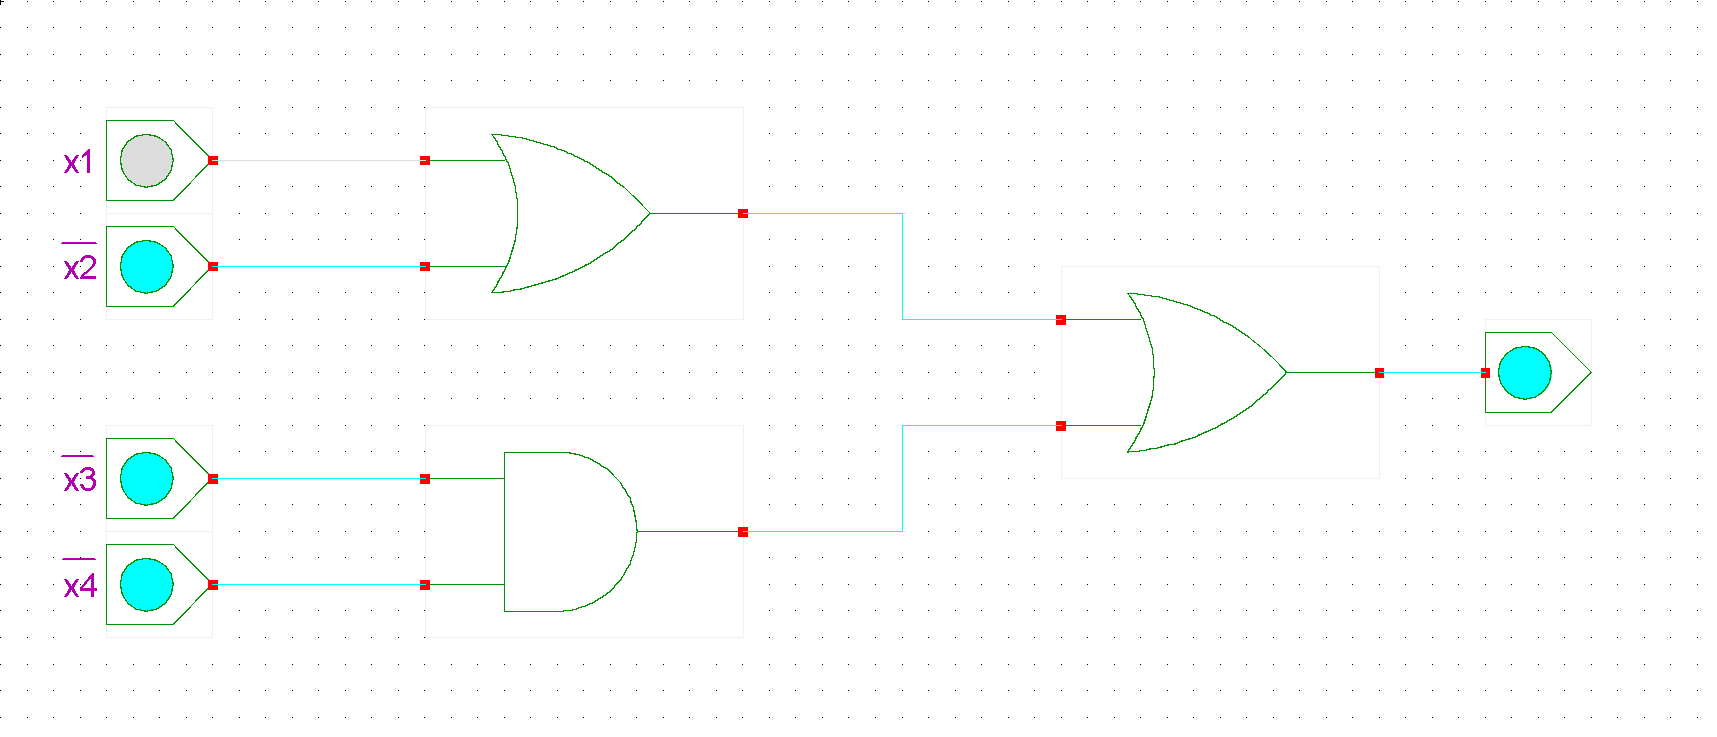
\includegraphics[width=0.8\textwidth]{disjunktiveform.PNG}

            Konjunktiveform:
            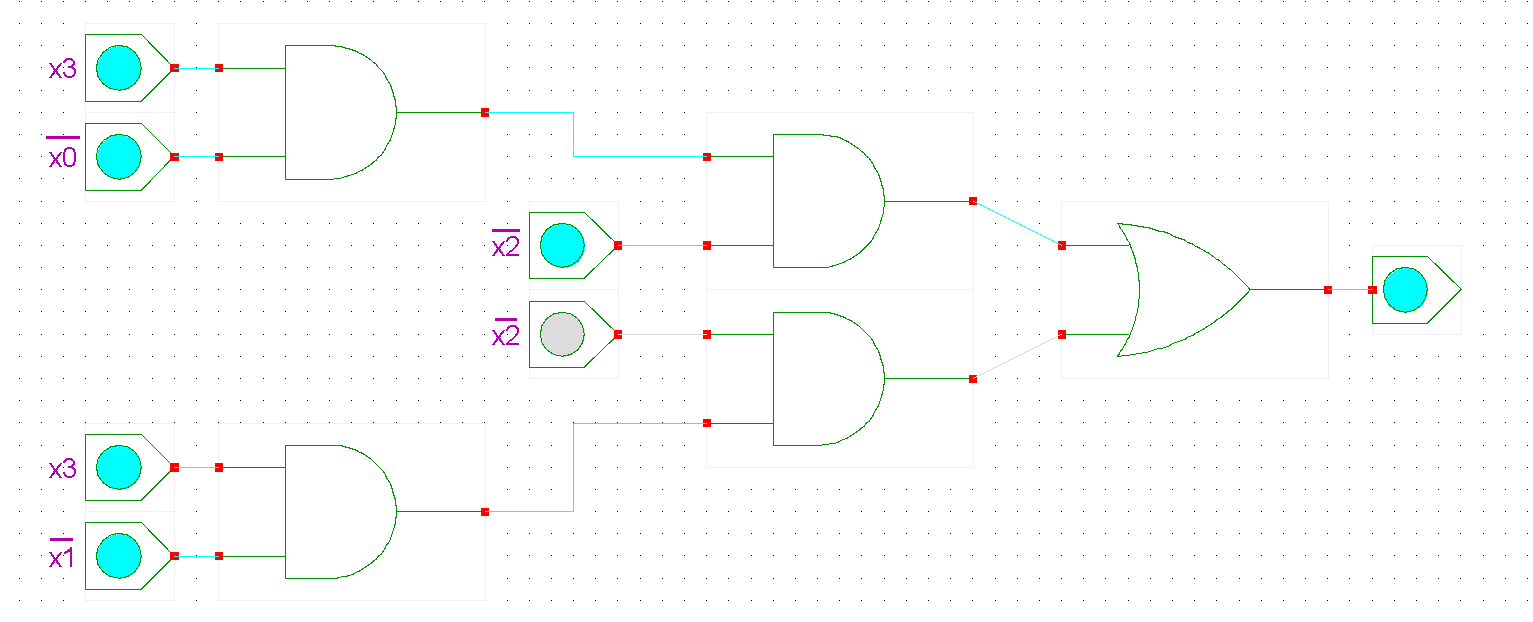
\includegraphics[width=0.8\textwidth]{knf.PNG}

    \end{enumerate}
    \item[\textbf{3.}]
        \begin{enumerate}
        \item[a)] Impulsdiagramm 1:

        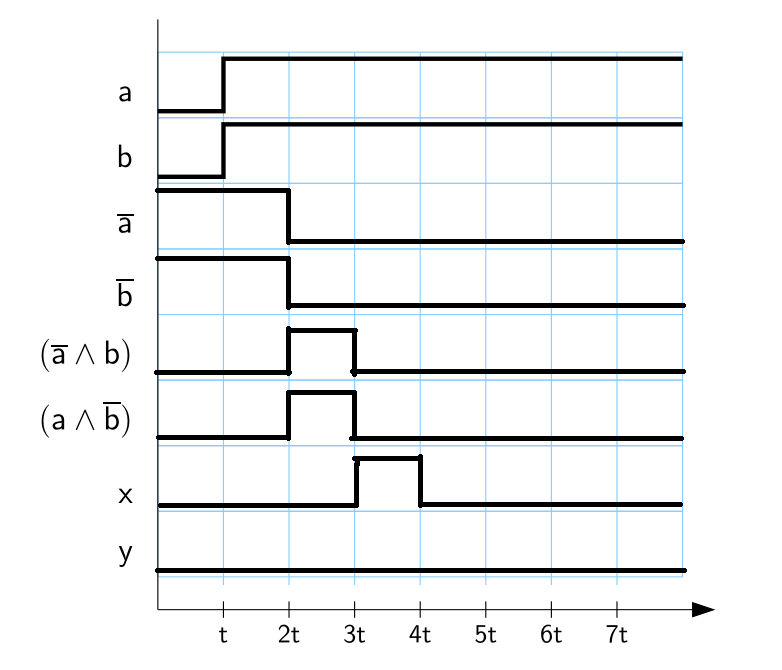
\includegraphics[width=0.5\textwidth]{3a.PNG}
        

        \item[b)] Impulsdiagramm 2:

        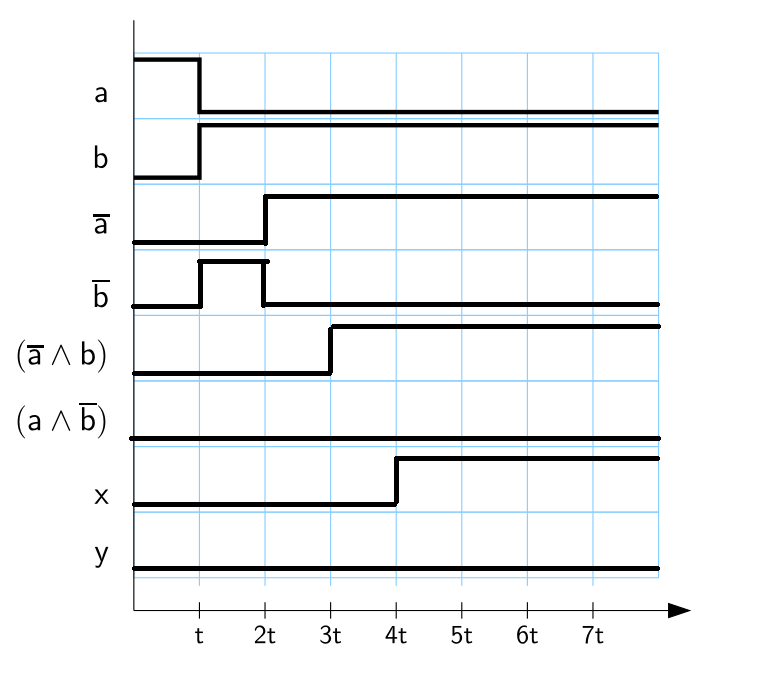
\includegraphics[width=0.5\textwidth]{3b.PNG}
        \end{enumerate}
    \item[\textbf{4.}]
        \begin{enumerate}
        \item[a)]
        \end{enumerate}
\end{enumerate}
\end{document}
